%!TEX encoding = UTF-8 Unicode

\documentclass{beamer}

\frenchspacing

\usepackage[utf8]{inputenc}
\usepackage[T1]{fontenc}
\usepackage[magyar]{babel}

% AMS
\usepackage{amssymb,amsmath}

% Graphic packages
\usepackage{graphicx}

% Syntax highlighting
\usepackage{listings}

\usepackage{caption}

\usepackage{array}
\newcolumntype{D}{>{\arraybackslash}m{0.3\textwidth}}
\newcolumntype{L}{>{\centering\arraybackslash}m{0.3\textwidth}}
\newcolumntype{Z}{>{\centering\arraybackslash}m{0.6\textwidth}}

\usetheme{Szeged}
\usecolortheme{beaver}

\title[IDE készítése a Rust-hoz]{Integrált fejlesztőkörnyezet készítése a Rust programozási nyelvhez}
\author{Varga Dániel}
\institute{Miskolci Egyetem}
\date{2019. június 12.}

\begin{document}
    \frame{\titlepage}

    \section{Rust}

    \subsection{A Rust nyelv}

    \begin{frame}[fragile]
        \frametitle{A Rust nyelv}

        \begin{itemize}
            \item Multi-paradigmájú rendszerprogramozási nyelv
            \item Biztonságos kódra helyez hangsúlyt
            \item Szintaktikailag hasonlít a C++-ra \begin{itemize}
                \item Tervezésben különbözik
                \item Memória-biztonság C++-hoz hasonló sebességek mellett
            \end{itemize}
            \item Cargo: NPM-hez hasonló csomag-menedzser
        \end{itemize}

    \end{frame}

    \begin{frame}[fragile]
        \frametitle{Történet}

        \begin{itemize}
            \item \textbf{2006:} Graydon Hoare, Mozilla alkalmazott személyes projektje
            \item \textbf{2009:} Mozilla támogatja a projektet \begin{itemize}
                \item Létrejön egy csapat, cél: \begin{itemize}
                    \item A nyelv tovább fejlesztése
                    \item A nyelv felhasználása Mozilla Servo projektjében
                \end{itemize}
            \end{itemize}
            \item \textbf{2010:} Mozilla nyilvánosságra hozza a nyelvet \begin{itemize}
                \item A csapat fókuszt vált
                \item Az eredeti OCaml-ben íródott fordító helyett írnak egy Rust fordítót Rust-ban (\texttt{rustc})
                \item LLVM backend-ként
            \end{itemize}
            \item \textbf{2011:} A \texttt{rustc} lefordítja saját magát
            \item \textbf{2012:} Első számozott pre-alfa kiadás
            \item \underline{\textbf{2015. május 15:}} Rust 1.0, nyelv és fordító kiadása \begin{itemize}
                \item Új verziók hat hetente
                \item Három csatornán: alfa, béta, és kiadás
            \end{itemize}
        \end{itemize}
    \end{frame}

    \begin{frame}[fragile]
        \frametitle{Összehasonlítás C++-szal}

        \begin{table}
            \centering
            \begin{tabular}{|D|L|L|}
                \cline{2-3}
                 \multicolumn{1}{c|}{} & Rust & C++ \\ \hline
                 Költség nélküli absztrakció & \multicolumn{2}{|Z|}{Igen: Trait / template dispatchelhető statikusan} \\ \hline
                 Mozgatás szemantika: forrásobjektumok állapota 
                 & Beépített statikus analizáló megtiltja az objektumok használatát mozgatás után 
                 & Javasolt, hogy egy mozgatás konstruktor érvényes állapotban hagyja a forrásobjektumot (de attól azt még nem érdemes használni) \\ \hline
            \end{tabular}
        \end{table}
    \end{frame}

    \begin{frame}[fragile]
        \frametitle{Összehasonlítás C++-szal}

        \begin{table}
            \centering
            \begin{tabular}{|D|L|L|}
                \cline{2-3}
                 \multicolumn{1}{c|}{} & Rust & C++ \\ \hline
                 "Használat mozgatás után" hibák 
                 & A fordító a fent említett analizálót használja ezek észrevételére 
                 & Felderíthetőek különleges "sentinel" állapottal futásidőben, vagy külsős kódellenőrző programokkal fordításidőben \\ \hline
                 "Használat felszabadítás után" hibák
                 & \multicolumn{2}{|Z|}{Okos mutatók használata ajánlott a nyers mutatók helyett ezek elkerülésére} \\ \hline
            \end{tabular}
        \end{table}
    \end{frame}

    \section{IDE}

    \subsection{Integrált fejlesztői környezetek}

    \begin{frame}[fragile]
        \frametitle{Integrált fejlesztői környezet}

        \begin{itemize}
            \item Az angol \emph{integrated development environment} (IDE) megnevezésből
            \item Gyakori IDE funkciók: \begin{itemize}
                \item Kódszerkesztés, kód színezése kontextus alapján
                \item Kódjavaslatok
                \item Kódellenőrzés, fordítás IDE-n belül
                \item Debuggolási lehetőségek
                \item Projektkezelés
            \end{itemize}
        \end{itemize}

    \end{frame}

    \begin{frame}[fragile]
        \frametitle{IDE-k a Rust nyelvhez}

        \begin{itemize}
            \item Eredetileg a nyelvfejlesztők tervei között volt
            \item Most: nyelvszerver (\emph{Rust Language Server}, RLS), amit IDE-k felhasználhatnak
            \item Létező Rust IDE-k: \begin{itemize}
                \item SolidOak \begin{itemize}
                    \item Github oldal archiválva
                \end{itemize}
                \item Ride \begin{itemize}
                    \item C++-ban íródott 
                    \item Fejlesztés abbamaradt
                    \item A fejlesztő szeretné Rust-ban újraírni a projektet, de nem talált megfelelő UI könyvtárakat a fejlesztéshez
                \end{itemize}
            \end{itemize}
            \item Jelenlegi helyzet: nincs Rust IDE
        \end{itemize}

    \end{frame}

    \begin{frame}[fragile]
        \frametitle{Minimális specifikáció}

        \begin{itemize}
            \item GTK widgetkönyvtár \begin{itemize}
                \item \texttt{GtkSourceView} a kódszerkesztéshez
            \end{itemize}
            \item GDK ablakkezeléshez és billentyűparancs-észrevételhez
            \item Pango a szövegkiíratáshoz
            \item Keccak hash függvény szövegtartalom-összehasonlításhoz \begin{itemize}
                \item Hogy el tudjuk dönteni, hogy kell-e menteni a szerkesztett szöveget
            \end{itemize}
        \end{itemize}
    \end{frame}

    \begin{frame}[fragile]
        \frametitle{További követelmények}

        \begin{itemize}
            \item Kommunikáció Cargo-val \begin{itemize}
                \item Szinkron processzmeghívás
            \end{itemize}
            \item Kommunikáció RLS-sel \begin{itemize}
                \item Rust forráskód szükséges
                \item Lecserél néhány Cargo parancsot, amik csak a \texttt{rustc}-t hívják meg (build, run, check, ...)
                \item Két megoldás: \begin{itemize}
                    \item RLS szerver futtatása a háttérben: aszinkron processzmeghívás
                    \item Ekkor \texttt{serde-json} a Kommunikációhoz
                    \item Az RLS \texttt{json-rpc} protokoll alapján kommunikál
                    \item Vagy: az RLS, mint könyvtár, beépítése a programba
                \end{itemize}
            \end{itemize}
        \end{itemize}
    \end{frame}

    \section{Minimális program}

    \subsection{Megvalósítás: minimális program}

    \begin{frame}[fragile]
        \frametitle{A Rozsda IDE}

        \begin{center}
            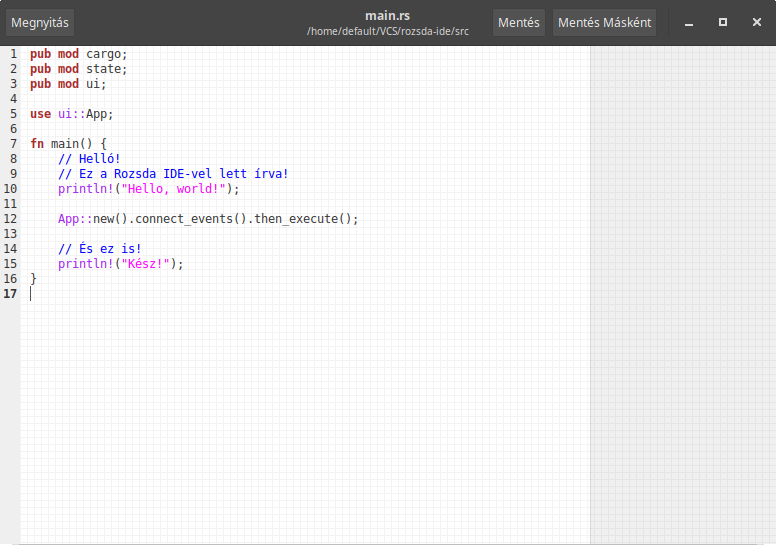
\includegraphics[scale=0.3]{kepek/mvp.png}
        \end{center}
    \end{frame}

    \begin{frame}[fragile]
        \frametitle{Cargo.TOML}

        \begin{itemize}
            \item A projekt mivoltját magyarázza
            \item Általában a \texttt{crates.io}-ra való feltöltéskor érdemes használni
            \item Ebben az esetben nem olyan fontos
            \item \texttt{edition = 2018}
            \item Megadjuk a függőségeket a \texttt{[dependencies]} kategóriában \begin{itemize}
                \item \texttt{gtk} és \texttt{sourceview} esetén a minimális GTK verziót is
            \end{itemize}
        \end{itemize}
    \end{frame}

    \begin{frame}[fragile]
        \frametitle{Cargo.TOML}

        \begin{lstlisting}
            [package]
            name = "rozsda-ide"
            version = "0.0.1"
            authors = ["Varga Daniel"]
            edition = '2018'
            
            // ...
            
            [dependencies.gtk]
            features = ["v3_22"]
            version = "0.6.0"
        \end{lstlisting}
    \end{frame}

    \begin{frame}[fragile]
        \frametitle{Az UI modul}

        \begin{itemize}
            \item \texttt{ui.rs} fájl
            \item Nem tartalmaz igazából kódot
            \item Szerepe: az \texttt{ui} modul definiálása, és a mélyebben lévő, fontosabb struktúrák és metódusok újra-exportálása
            \item Újra-exportálás: Nyilvános metódust vagy struktúrát (vagy akár modult) a \texttt{use} paranccsal behívunk a jelenlegi modulba \begin{itemize}
                \item Cél: az elérési útvonal rövidítése
                \item Pl.: ha az \fbox{\texttt{egyik::masik::harmadik::Negyedik}} struktúrát meghívjuk az \texttt{egyik}-ben \fbox{\texttt{pub use self::masik::harmadik::Negyedik}} paranccsal,
                akkor az elérhető lesz \fbox{\texttt{egyik::Negyedik}}-ként is 
            \end{itemize}
        \end{itemize}
    \end{frame}

    \begin{frame}[fragile]
        \frametitle{Az \texttt{App}}

        \begin{itemize}
            \item Egyelőre csak felépít egy GTK ablakot
            \item GTK inicializálása, ablak példányosítása és beállítása
            \item Tartalmazza a létrehozott ablakot
            \item Rust lexikai zárványa: \texttt{move |\_, \_| \{\dots\}}
            \begin{itemize}
                \item Gyakori a GTK használatakor
                \item Ebben az esetben: a paraméter-metódusnak két paramétere van
                \item A zárvány birtokolni fogja a paramétereket (\texttt{move})
                \item Paraméterek megadása: \texttt{|param1, param2, \dots|}
                \item Nem akarunk semmit tenni az átadott paraméterekkel, így névtelenként adjuk meg őket (\texttt{\_})
            \end{itemize}
        \end{itemize}
    \end{frame}

    \begin{frame}[fragile]
        \frametitle{A fejléc, \texttt{Header}}

        \begin{itemize}
            \item \texttt{HeaderBar} GTK elem
            \item Egyelőre a fő gombokat tartalmazza (Megnyitás, Mentés, Mentés Másként)
            \item Újra-exportálás: \fbox{\texttt{pub use self::header::Header;}} az \texttt{ui.rs}-ben
            \item Kibővítjük az \texttt{App}-ot, hogy tartalmazzon egy \texttt{Header}-t
            \item Fejléc beállítása az ablakhoz: \fbox{\texttt{window.set\_titlebar(\&header.container);}}
        \end{itemize}
    \end{frame}

    \begin{frame}[fragile]
        \frametitle{A kódszerkesztő, \texttt{SourceView}}

        \begin{itemize}
            \item \texttt{Source} struktúra \begin{itemize}
                \item Tartalmazza a \texttt{SourceView}-et és a pufferjét
                \item Tartalmaz egy \texttt{ScrolledWindow}-t, hogy a kódszerkesztő rész görgethető legyen
                \item Beállítja a \texttt{SourceView}-et, hogy a Rust nyelvhez igazodjon, illetve hogy a mi általunk megadott puffert használja 
            \end{itemize}
            \item \texttt{Content} struktúra \begin{itemize}
                \item "Becsomagolja" a \texttt{Source}-t
                \item Később kibővíthetjük a kódszerkesztő részt, ha szükséges (pl. több fájl egyszerre megnyitva)
            \end{itemize}
        \end{itemize}
    \end{frame}

    \begin{frame}[fragile]
        \frametitle{\texttt{ActiveMetadata}}

        \begin{itemize}
            \item A mentéshez szükséges eldönteni, hogy egyáltalán hol is van a fájlunk, és mi a tartalma
            \item Ez az \texttt{ActiveMetadata} szerepe
            \item Tartalma: útvonal puffer a fájl helyének, és egy 64 elemes 8-bit hosszú elemeket tartalmazó tömb
            \item Az utóbbi: 512 rátás Keccak algoritmus hash szummát tartalmaz \begin{itemize}
                \item Megnyitáskor kiszámítjuk a megnyitott fájl tartalmának a hash-jét
                \item Fájl szerkesztés során összehasonlítjuk a \texttt{SourceView} pufferének tartalmának hash-jével
                \item Ha nem egyezik meg: mentetlen módosítások
            \end{itemize}
        \end{itemize}
    \end{frame}

    \begin{frame}[fragile]
        \frametitle{\texttt{Option}: a Rust \texttt{null}-ja}

        \begin{itemize}
            \item A \texttt{PathBuf} kezelésénél megjelenik az \texttt{Option}
            \item A \texttt{null} megfelelője a Rust-ban
            \item Tiltott a null mutató
            \item Helyette az \texttt{Option} fejezi ki annak lehetőségét, hogy lehet inicializálatlan egy változó  
            \item Az \texttt{Option<T>} egy enumeráció, aminek értéke lehet: \begin{itemize}
                \item \texttt{Some<T>}: A \texttt{T} típusú belső érték létezik, beépített metódusokkal megszerezhető
                \item \texttt{None}: A \texttt{T} típusú belső érték nem létezik
            \end{itemize}
        \end{itemize}
    \end{frame}

    \begin{frame}[fragile]
        \frametitle{A felugró ablakok}

        \begin{itemize}
            \item A GTK-s elemek nem pusztulnak el akkor, amikor elvárnánk
            \item Szükséges manuálisan elpusztítani őket
            \item Ez inkább a felugró ablakoknál releváns, hiszen más elemeket nem hozunk létre és pusztítunk el annyiszor a program során
            \item Egyszerűbb megoldás: a \texttt{Drop} tulajdonságot implementáljuk egy \texttt{FileChooserDialog}-ot becsomagoló struktúránkba
            \item Létrehozunk saját struktúrákat, amik beállítják a felugró ablakot
            \item \texttt{OpenDialog}, \texttt{SaveDialog}
        \end{itemize}
    \end{frame}

    \begin{frame}[fragile]
        \frametitle{Mentés: \texttt{SaveAction}}

        \begin{itemize}
            \item A mentés sikerességének leírására létrehozunk egy \texttt{SaveAction} enumerációt \begin{itemize}
                \item \texttt{New(ActiveMetadata)}: a fájlt másként mentettük (vagy nem volt betöltve fájl, és először mentünk), és belső értékként visszakapjuk a mentett fájl adatait
                \item \texttt{Saved}: a fájlt sikeresen mentettük
                \item \texttt{Canceled}: a felhasználó kilépett a mentés felugró ablakból, vagy valamiért nem sikerült a mentés
            \end{itemize}
            \item Ezt felhasználjuk a kiíratás metódusban
        \end{itemize}
    \end{frame}

    \begin{frame}[fragile]
        \frametitle{Mentés: kiíratás}

        \begin{block}{Kiíratás metódusa}
            \texttt{fn write\_data(path: Option<\&ActiveMetadata>, data: \&[u8]) -> io::Result<SaveAction>}
        \end{block}

        \begin{itemize}
            \item A metódus kiírja az \texttt{ActiveMetadata} által megadott fájlba a \texttt{SourceView} pufferének tartalmát
            \item Ha nem létezik az \texttt{ActiveMetadata}, akkor egy \texttt{SaveDialog}-gal megkéri a felhasználót, hogy válasszon mentési helyet, és az alapján készít egyet
            \item A \texttt{data} paraméter a \texttt{SourceView} pufferének tartalma
            \item Visszatérési érték egy \texttt{Result}-ba csomagolt \texttt{SaveAction}
        \end{itemize}
    \end{frame}

    \begin{frame}[fragile]
        \frametitle{\texttt{Result}: az \texttt{Option} testvére}

        \begin{itemize}
            \item A \texttt{Result} a kivételkezelés megfelelője a Rust-ban
            \item A \texttt{Result<T, E>} enumerációnak két változata van: \begin{itemize}
                \item \texttt{Ok<T>}: sikeresen megtörtént, amit tenni akartunk, és visszakapjuk a \texttt{T} típusú belső értéket
                \item \texttt{Err<E>}: sikertelen volt a metódus, és egy \texttt{E} típusú hibaértéket kaptunk vissza
            \end{itemize}
            \item \textbf{De}: az előbb csak \texttt{io::Result<SaveAction>}-t adtunk meg \begin{itemize}
                \item Szokás a Rust programozók között a \texttt{Result} felüldefiniálása, ha egy modul várhatóan mindig ugyanazzal a hibával tér vissza
                \item Az \texttt{io::Result} definíciója: \fbox{\texttt{pub type Result<T> = result::Result<T, Error>;}}
                \item Mivel az \texttt{io} modul várhatóan input-output hibákkal fog visszatérni, ezért a Rust fejlesztői így definiálták az \texttt{io::Result}-ot kényelmi okokból
            \end{itemize}
        \end{itemize}
    \end{frame}

    \begin{frame}[fragile]
        \frametitle{Mentés: a mentés metódus}

        \begin{itemize}
            \item Egyszerű
            \item A \texttt{write\_data()}-nak továbbítjuk a szükséges paramétereket
            \item Ha kell, frissítjük a fejlécet és legeneráljuk a fájl új hash-ját
            \item Vagy lecseréljük a jelenlegi \texttt{ActiveMetadata}-t a \texttt{write\_all()} által szolgáltatottra
            \item Vagy nem teszünk semmit
        \end{itemize}
    \end{frame}

    \begin{frame}[fragile]
        \frametitle{A program összekapcsolása}

        \begin{itemize}
            \item A GTK elemek kibocsátanak jelzéseket, ha történik velük valami
            \item Pl.: a gombok \texttt{connect\_clicked()} jelzése meghívja a paraméterként megadott metódust, ha a felhasználó megnyomja a gombot
            \item Az \texttt{App} \texttt{save\_event()} metódusában kössük össze a Mentés és Mentés Másként gombokat a \texttt{save()} metódusunkkal
        \end{itemize}
    \end{frame}

    \begin{frame}[fragile]
        \frametitle{A program összekapcsolása}

        \begin{block}{Az \texttt{App} \texttt{save\_event()} metódusa}
            \begin{lstlisting}
let editor = self.content.source.buff.clone();
let headerbar = self.header.container.clone();
let save_button = save_button.clone();
actual_button.connect_clicked(move |_| {
    save(&editor, &headerbar, &save_button, 
    &current_file, save_as)
});
            \end{lstlisting}
        \end{block}

        \begin{itemize}
            \item Nem tűnik helyes kódnak, de a Rust fordító mégis elfogadja
            \item Miért?
        \end{itemize}
    \end{frame}

    \begin{frame}[fragile]
        \frametitle{A \texttt{Clone} tulajdonság}

        \begin{itemize}
            \item A legtöbb GTK elem implementálja a \texttt{Clone} tulajdonságot
            \item Ez lehetőséget ad a \texttt{clone()} metódus meghívására
            \item Klónozás = másolás, az eredeti és a klón értékeikben megegyeznek, de különböző példányok
            \item Tehát az előző kódnak nem is szabadna működnie \begin{itemize}
                \item Minden elemet klónozunk
                \item Soha nem tudnánk leellenőrizni, hogy az "eredeti" gomb le lett-e nyomva, például
            \end{itemize}
            \item A GTK megszegi a klónozás szabályait?
        \end{itemize}
    \end{frame}

    \begin{frame}[fragile]
        \frametitle{A GTK objektumai}

        \begin{itemize}
            \item \textbf{Nem} (teljesen), a furcsának tűnő kód a GTK felépítéséből jön
            \item Valójában a Rust-os GTK objektumok csak mutatók a Rust alatt futó C-s GTK-s objektumokra
            \item A GTK magának szemétgyűjtő rendszert is fenntart
            \item Bár a GTK sok Rust szabályt megszeg, a klónozásét nem (a mutató értéke helyesen átmásolódik a klónba is)
            \item Innen jön az is, hogy manuálisan kellett megszüntetnünk a felugró ablak létezését \begin{itemize}
                \item Amíg a szülő ablak (a fő ablak) él, addig a felugró ablak nem szűnik meg
            \end{itemize}
        \end{itemize}
    \end{frame}

    \begin{frame}[fragile]
        \frametitle{Az összekapcsoltság biztosítása}

        \begin{itemize}
            \item Hogyan biztosítsuk, hogy az \texttt{App} elemeinek minden relevánsz szignálja kapcsolva legyen egy metódushoz?
            \item Megoldás: \texttt{ConnectedApp} \begin{itemize}
                \item Becsomagolja az \texttt{App}-ot
                \item Új metódus az \texttt{App}-ban, \texttt{connect\_events()}, ami létrehoz egy \texttt{ConnectedApp}-ot, és átadja neki saját magát
                \item Nincs \texttt{new()} metódus a \texttt{ConnectedApp}-ban: csak a fenti metódussal hozható létre
            \end{itemize}
            \item Előny: tudjuk, mikor jeleníthetjük meg az ablakot, mikor van az "készen"
        \end{itemize}
    \end{frame}

    \section[Cargo parancsok]{cargo}
    \subsection{Megvalósítás: Cargo parancsok hívása a programból}

    \begin{frame}[fragile]
        \begin{center}
            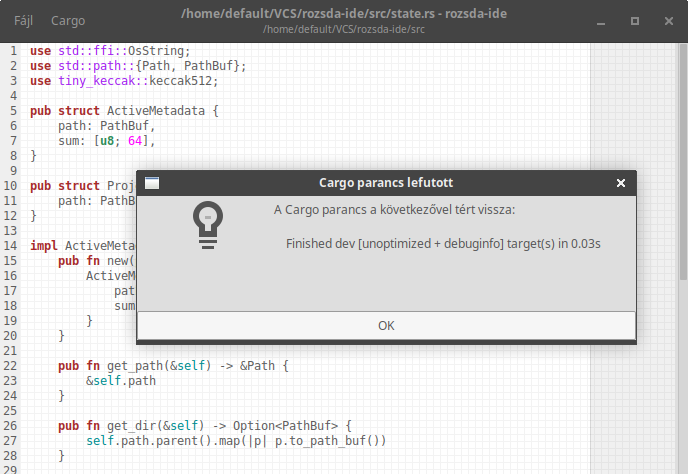
\includegraphics[scale=0.3]{kepek/cargo.png}
        \end{center}
    \end{frame}

    \begin{frame}[fragile]
        \frametitle{A \texttt{Header} átrendezése}

        \begin{itemize}
            \item Gombok helyett \texttt{MenuItem}-ek
            \item Lehetővé teszi a menük behozatalát
            \item A fejléc címmódosítása átkerül ide \begin{itemize}
                \item Ehhez kap egy \texttt{Arc<RwLock<Option<ActiveMetadata>{}>{}>} adattagot, ami az \texttt{ActiveMetadata}-ra mutathat
            \end{itemize}
            \item Az eddigi gombokat "átmozgatjuk" a Fájl menübe
            \item Az új Cargo menübe kerülnek majd a Cargo műveletek
        \end{itemize}
    \end{frame}

    \begin{frame}[fragile]
        \frametitle{Projektkezelés}

        \begin{itemize}
            \item Létrehozunk egy \texttt{ProjectMetadata}-t a projektek kezelésére \begin{itemize}
                \item Egyszerűbb, mint az \texttt{ActiveMetadata}: csak a projekt elérési útvonala szükséges
                \item Nem szükséges fájlkezelés
                \item Ezt adjuk át a Cargo parancsoknak
            \end{itemize}
            \item Ezek mellett új felugró ablakok: \texttt{OpenFolderDialog} és \texttt{CreateFolderDialog} \begin{itemize}
                \item Csak abban különböznek a meglévőktől, hogy könyvtárakat kezelnek fájlok helyett
            \end{itemize}
        \end{itemize}
    \end{frame}

    \begin{frame}[fragile]
        \frametitle{A kód leegyszerűsítése}

        \begin{itemize}
            \item Az \texttt{App} tartalmazza \texttt{Arc<RwLock<Option<{}>{}>{}>}-ba csomagolva mind az \texttt{ActiveMetadata}-t, mind a \texttt{ProjectMetadata}-t
            \item Miért egyszerűbb? \begin{itemize}
                \item Mindkettő addig él, amíg a program is, és az \texttt{App} írja le a programot
                \item \texttt{Option}: lehet, hogy nem nyitottunk meg még fájlt / projektet
                \item \texttt{RwLock}: írás-olvasásra specializálódott zár, vagy egy író, vagy végtelen olvasó
                \item \texttt{Arc}: referencia számolt, szálbiztos okos mutató
            \end{itemize}
        \end{itemize}
    \end{frame}

    \begin{frame}[fragile]
        \frametitle{Cargo parancsok}

        \begin{block}{A Cargo parancsok formája általában}
            \begin{lstlisting}
pub fn check_cargo_project(location: &Path)
-> std::io::Result<process::Output>
{
    process::Command::new("cargo")
    .current_dir(location)
    .args(&["check", "--message-format", "short"])
    .output()
}
            \end{lstlisting}
        \end{block}
    \end{frame}

    \begin{frame}[fragile]
        \frametitle{Cargo parancsok}

        \begin{itemize}
            \item Minden Cargo parancsnak (build, run, check, clean, test) írunk egy metódust
            \item Egy enumeráció felhasználásával eldönthetjük, melyiket hívjuk éppen meg
            \item Egy összekapcsoló meghívó metódus az enumeráció alapján dönti el, hogy melyik Cargo parancsot hívja meg 
        \end{itemize}
    \end{frame}

    \section{Tesztek}
    \subsection{Tesztek, eredmények}

    \begin{frame}[fragile]
        \frametitle{Mentetlen, névtelen fájl}

        \begin{center}
            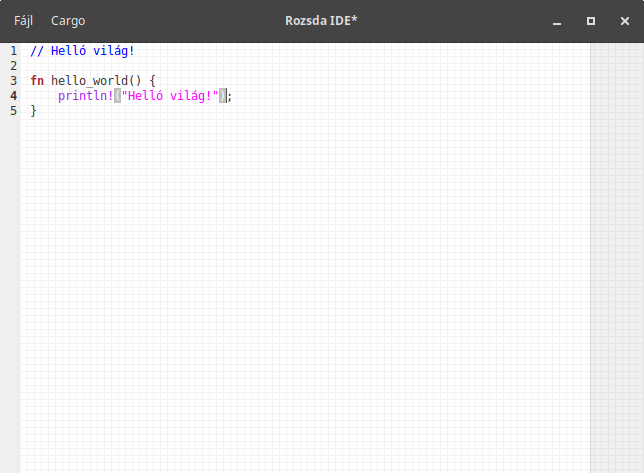
\includegraphics[scale=0.3]{kepek/nevtelen-fajl.png}
        \end{center}
    \end{frame}

    \begin{frame}[fragile]
        \frametitle{Elmentett fájl}

        \begin{center}
            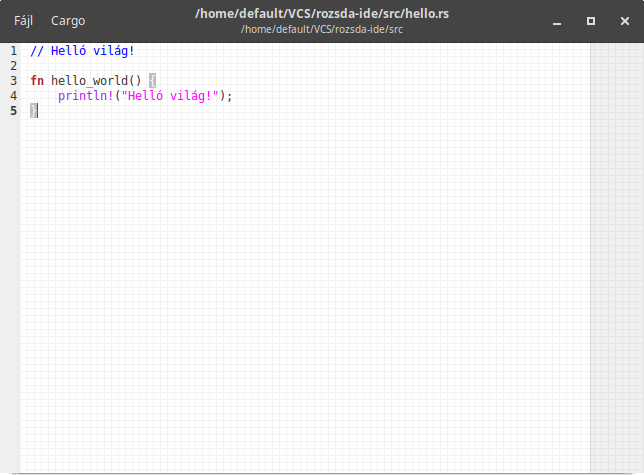
\includegraphics[scale=0.3]{kepek/elmentett-fajl.png}
        \end{center}
    \end{frame}

    \begin{frame}[fragile]
        \frametitle{Fájl bezárása / kilépés mentetlen változásokkal}

        \begin{center}
            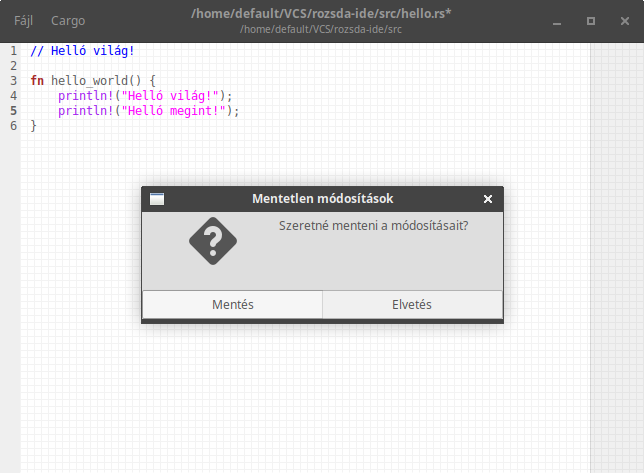
\includegraphics[scale=0.3]{kepek/kilepes-mentetlen-valtozasokkal.png}
        \end{center}
    \end{frame}

    \begin{frame}[fragile]
        \frametitle{Projekt megnyitása}

        \begin{center}
            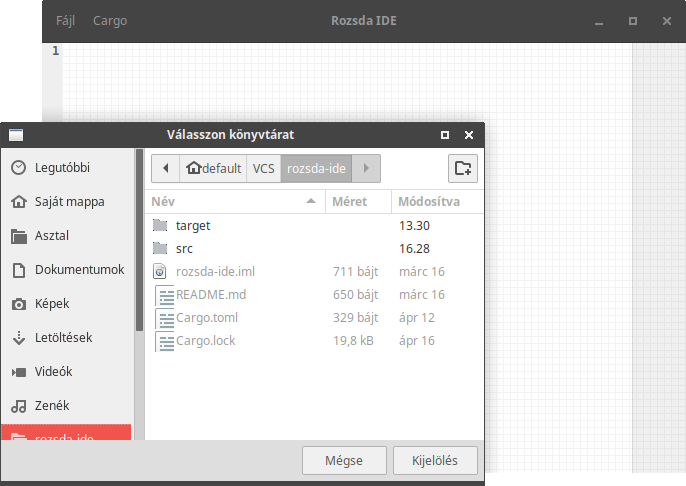
\includegraphics[scale=0.3]{kepek/projekt-megnyitas.png}
        \end{center}
    \end{frame}

    \begin{frame}[fragile]
        \frametitle{Projekt megnyitás sikeres}

        \begin{center}
            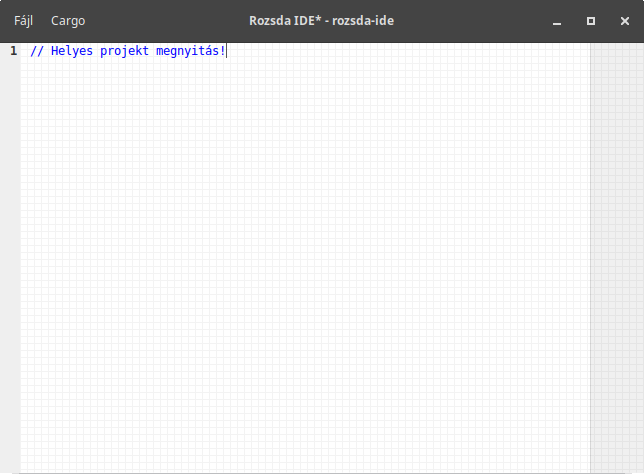
\includegraphics[scale=0.3]{kepek/projekt-megnyitas-sikeres.png}
        \end{center}
    \end{frame}

    \begin{frame}[fragile]
        \frametitle{Projekt megnyitás sikertelen}

        \begin{center}
            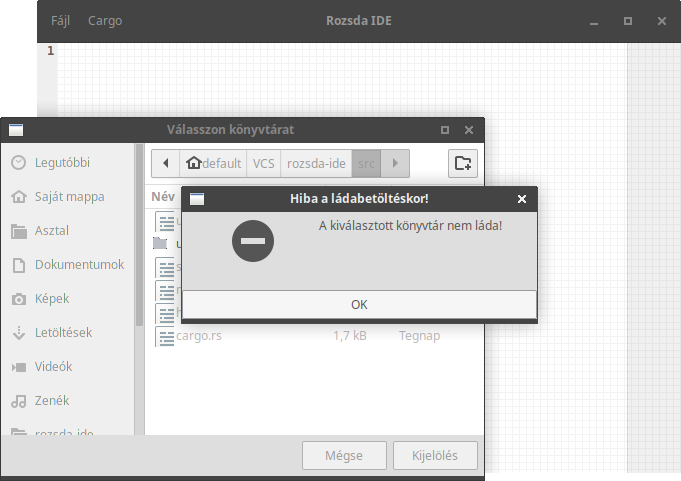
\includegraphics[scale=0.3]{kepek/projekt-megnyitas-sikertelen.png}
        \end{center}
    \end{frame}

    \begin{frame}[fragile]
        \frametitle{Rozsda IDE megnyitása Rozsda IDE-ben}

        \begin{center}
            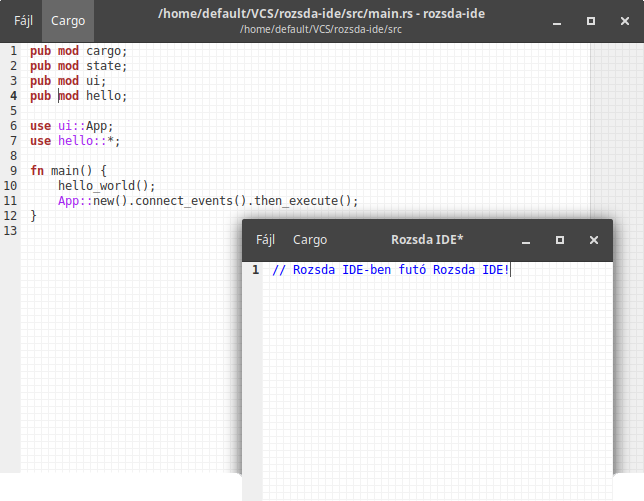
\includegraphics[scale=0.3]{kepek/rozsda-ide-rozsda-ideben.png}
        \end{center}
    \end{frame}

    \section{Összegzés}
    \subsection{Összegzés}

    \begin{frame}[fragile]
        \frametitle{Új tapasztalatok}

        \begin{itemize}
            \item Megismerkedtem a Rust nyelvvel
            \item Megismerkedtem a GTK használatával, mint fejlesztő (felhasználóként már használtam)
            \item Sokat tanultam a fejlesztői környezetekről
        \end{itemize}
    \end{frame}

    \begin{frame}[fragile]
        \frametitle{Nehézségek}

        \begin{itemize}
            \item A Rust "front heavy" nyelv: nehezen lehet eljutni egy minimális megfelelő programhoz, de onnantól könnyebb a programozás
            \item A GTK binding-ek nem tartották be a Rust szabályait
            \item Hiányos vagy félrevezető dokumentáció
        \end{itemize}
    \end{frame}

    \begin{frame}[fragile]
        \begin{center}
            \Large \textbf{Köszönöm a figyelmet!}
        \end{center}
    \end{frame}
\end{document}
